\chapter{Relations}

Given two classes \(A\) and \(B\), a \emph{relation} \(R\) is a subset of its \emph{Cartesian product} \(R \subseteq A \times B\). 

\textbf{Example:} 

Given \(A = \{1,2,3\}\) find the elements of the relation \(R\) defined by \(R = \{(a, b) \in A \times A \mid a < b\}\).

\[
	A \times A = \{(1,1), (1,2), (1,3), (2,1), (2,2), (2,3), (3,1), (3,2), (3,3)\}
\]

The relation \(R\) would then be:

\[
	R = \{(1,2), (1,3), (2,3)\}
\]

Common types of relations include:

\begin{itemize}

	\item \emph{Functions}: special relations where each input has exactly one output.

	\item \emph{Equivalence relations}: reflexive, symmetric, and transitive.

	\item \emph{Partial orders}: reflexive, antisymmetric, and transitive.

\end{itemize}

\subsection{Types of Relations}

Let \(A\) be a set and \(X\) be a relation on \(A\).

\begin{itemize}

	\item \emph{Reflexive:} \(\forall a \in A: (a, a) \in X\) (or written as \(a \sim a\))

	\item \emph{Irreflexive:} \(\forall a \in A: (a, a) \not\in X\)

	\item \emph{Symmetric:} \(\forall a, b \in A: (a, b) \in X \to (b, a) \in X\) (or written as 
		  \((a \sim b) \Rightarrow (b \sim a)\))

	\item \emph{Antisymmetric:} \(\forall a, b \in A: (a, b) \in X \text{ and } (b, a) \in X \implies a = b\)

	\item \emph{Transitive:} \(\forall a, b, c \in A: (a, b) \in X \text{ and } (b, c) \in X \to (a, c) 
		  \in X\) (or written as \((a \sim b) \text{ and } (b \sim c) \Rightarrow (a \sim c)\))

	\item \emph{Total:} \(\forall a,b \in A: a \neq b \to (a, b) \in X \text{ or } (b, a) \in X\)

\end{itemize}

\section{Diagonal Graph}

Given a relation, the \emph{graph} \(I_A\) is defined as 

\[
	\{(x, x) \mid x \in A\}
\] 

and is denoted as the \emph{diagonal graph} of \(A\).

\subsection{Lemmas for Proofs}

Let the graph \(G\) be a relation on \(A\).

\begin{itemize}
	
	\item \(G\) is symmetric if and only if \(G = G^{-1}\).

	\item \(G\) is antisymmetric if and only if \(G \cap G^{-1} \subseteq I_A\).

	\item \(G\) is transitive if and only if \(G \circ G \subseteq G\).

\end{itemize}

\section{Order Relation}

A relation is called an \emph{order relation} \(R \subseteq A \times A\) if it is \emph{reflexive}, \emph{antisymmetric} and \emph{transitive}.

\subsection{Inverse Order Relation}

Given an order relation \(G\) on \(A\), then \(G^{-1}\) is also an order relation on \(A\).

\subsection{Strict Order Relation}

A relation is called a \emph{strict order relation} \(R \subseteq A \times A\) if it is \emph{irreflexive}, \emph{antisymmetric} and \emph{transitive}.

\subsection{Inverse Strict Order Relation}

Given a strict order relation \(G\) on \(A\), then \(G^{-1}\) is also a strict order relation on \(A\).

\section{Equivalence Relation}

An \emph{equivalence relation} is a relation \(R \subseteq A \times A\) that is \emph{symmetric}, \emph{transitive} and \emph{reflexive}.

\textbf{Example:}

\[
	R:= \{ (a,b) \in \N \times \N: a = b\}
\]

\subsection{Properties of Equivalence Relations}

Given the equivalence relations \(G\) and \(H\), the following properties apply:

\begin{itemize}

	\item \(G \circ H\) is an E.R. if and only if \(G \circ H = H \circ G\).

	\item \(G \cup H\) is an E.R. if and only if  \(G \circ H \subseteq G \cup H \land H \circ G \subseteq G \cup H\).

\end{itemize}

\subsection{Inverse Equivalence Relation}

Given an equivalence relation \(G\) on \(A\), then \(G^{-1}\) is also an equivalence relation on \(A\).

\section{Equivalence Class}

Let \(R\) be an equivalence relation on a set \(A\) and \(a \in A\), the  \emph{equivalence class} of \(a\), denoted by 

\[
	[a]_R := \{y \in A \mid (a,y) \in R\}
\] 

is the set of all elements in \(A\) that are related to \(a\).

\subsection{Lemmas About Equivalence Classes}

For \(a,b \in A\) then 

\begin{itemize}

	\item \(aRb \iff [a]_R = [b]_R\)

	\item \(a \neg R b, (a,b) \notin R \iff [a]_R \cap [b]_R = \emptyset \)

\end{itemize}

\textbf{Proof I:}

\(aRb, x \in [a]_R \text{ tells us that also } x R b \implies x \in [b]_R \). For the other direction 
using the reflexive property we get \([a]_R = [b]_R \implies a R a \implies a \in [a]_R = [b]_R\).

\QED

\textbf{Proof II:}

\(x \in [a]_R \cap [b]_R \implies x R a, x R b, a R x \implies a R b\), a contradiction. 
Now, for \( [a]_R \cap [b]_R = \emptyset\) we can say \(a R b \implies a \in [a]_R, a \in [b]_R \), another contradiction.

\QED 

\section{Quotient Space}

Let \(R\) be an equivalence relation on a set \(A\). The \emph{quotient space} of \(A\) by 
\(R\), denoted by \(A / R\), is the set of all distinct equivalence classes of 
elements in \(A\). Formally, it is defined as:

\[
	A / R := \{[x]_R \mid x \in A\}
\]

The quotient space \(A/R\) is a partition of the original set \(A\) into disjoint equivalence classes. 
Each element of the quotient space is an equivalence class \([x]_R\), which itself is a subset of \(A\).

\subsection{Representative System of a Equivalence Relation}

Given an equivalence relation \(R\) on \(A\), a set  \(S \subseteq A\) which obeys that 

\[
	\forall a \in A, \!exists s \in S: a \in [s]_R
\]

we call this subset a \emph{representative system} of \(R\).

\subsection{The Quotient Is an Equivalence Relation}

The Quotient is an Equivalence Relation.

\textbf{Proof:}

\emph{Reflexivity}: For \(([x]_{G}, [y]_{G}) \in H/G\) we know claim that \([x]_{G} \sim [x]_{G}\). By the reflexivity 
of \(H\) we know that \(x \sim x\), which means that \((x, x) \in H\); and therefore, \([x]_{G} \sim [x]_{G}\). 

\emph{Symmetry}: For \(([x]_{G}, [y]_{G}) \in H/G\) we know claim that \(([x]_{G} \sim [y]_{G}) \land ([y]_{G} \sim [x]_{G})\). Analogously to our last property, 
if \((x \sim y) \land (y \sim x)\) were not true then \(H\) would not be an equivalence relation which leads to a contradiction of our initial conditions. Hence, 
the symmetric property is present.

\emph{Transitivity}: Lastly, the transitivity we again use the same argument as before using our base elements and pairs from \(H\) to arrive at a contradiction, which hich 
guarantees us that their equivalence class counterpart are also part of an equivalence relation..

\QED

\subsection{The Union of the Quotient Space}

Given \(A/R\), then \(\bigcup A/R = A\).

\textbf{Proof:}

Suppose \(a_0 \in A \land a_0 \notin [a]_R, \forall [a]_R \in A/R\). If \(R\) is an equivalence relation then 
\( a_0 \in A\) with \(R\) implies that \((a_0, a_0) \in R\). Therefore, the only way for \(a_0\) to not belong to any equivalence class is if \(R\)
were not an equivalence relation, which contradicts our initial condition; hence, we know that the union of the equivalence classes 
given an equivalence relation must be equal to the original set.

\QED

\subsection{Relation from the Relation of the Quotient Space and Partition from the Quotient Space}

Given \(R\) on \(A\), \(R_{A/R} = R\) with 

\[
	R_{A/R} = \{(a, b) \mid (a, b) \in A \times A, \exists X \in A/R, a,b \in X\}.
\]

And for \(S\) a partition of \(A\), then \(A/R_S = S\).

\textbf{Proof:}

For the first statement we need to prove the condition of an equivalence relation: 

\emph{Reflexivity}: \((a, b) \in R_{A/R} \implies a, b \in [x]_R \in A/R \implies a \sim x \land b \sim x \land a \sim b \land a \sim a \implies (a, a) \in R_{A/R}\).

\emph{Symmetry}: \((a, b), (b, a) \in R_{A/R} \implies a, b \in [x]_R \in A/R \implies a \sim x \land b \sim x \land a \sim b \land b \sim a \implies (a, b),(b,a) \in R_{A/R}\).

\emph{Transitivity}: \((a, b), (b, c) \in R_{A/R} \implies a, b \in [x]_R \in A/R \land b,c \in [y]_R \in A/R \implies a \sim x \land b \sim x \land b \sim y \land a \sim y \implies (a, b),(b,c),(a, c) \in R_{A/R} \).

Thus, \(R_{A/R} = R\). For the other direction \((a, b) \in R \implies b \in [a]_R \in A/R \implies a R_{A/R} b\)).

For the second part: \(A/R_S = S\):

Let \(S\) be a partition of \(A\), and \(X \in A/R_S\). For \(X = [a]_{R_S} = \{x \in A \mid a R_S x\}\). 
For \(a\) and \(b\) to be in a relation they need to be part of the same element \(Y \in S\). We need to prove that 
\(Y = [a]_{R_S}\). 

This is proven directly by the very definition of the relation \(R_S\) which implies that all elements belong to the same set \(Y\).
For the other direction if \(a, b \in Y \implies a E_S b \implies b \in [a]_{R_S} \in A/R_S\).

\QED

\section{Partitions}

Let \(A\) be a set. A \emph{partition} of \(A\) is a set of non-empty subsets in \(\mathcal{P}(A)\) with the following properties:

\[
	\forall i, j \in I A_i \cap A_j = \emptyset \quad \text{for} \quad i \neq j
\]

and 

\[
	\bigcup_{i \in I} A_i = A \quad \text{ or equivalently } \quad \bigcup_{i \in I} A_i \subseteq A
\]

\textbf{Example:}

Prove that \(B_n = \{m \in \Z \mid \exists q, m = n + 5q\}\) is a partition of \(\Z\). 

First, we prove the disjoint property, which means \(m \in B_x \land m \in B_y \iff x = y\).

For the union, we need to prove that every \(B_n\) is not empty, which is very easy by letting \(m = n + 5\cdot0 \implies m = n\); then 
combining all of them with the union will give us the entire set of integers, because each of the sets \(B_n\) has at least the number 
\(n\) in it, which can be any integer.

\QED

\subsection{Representatives}

Given a partition \(P\) of a set \(M\), the elements of \(P\) are called \emph{classes}. 
If \(X\) is a class, then its members are called \emph{representatives} of the class.

A subset of \(M\) with an element of each of the classes of \(M\) is called the \emph{representative set} or \emph{traversal}. 

The function \(v: P \to M\) with \(v(X) \in X\) for all \(X \in P\) is called \emph{representative function}.

\subsection{Properties of Partitions}

\begin{itemize}

	\item Every equivalence relation corresponds to a partition:

		  \[
		      J: \{ R : R \text{ is an equivalence relation on } X\} \to \{ F: F\ \text{is a partition of } X\}
	      \]

	      where \( J(R) := X / R \) is a bijection.

	\item If \(F\) is a partition of \(X\), then we can define an equivalence relation \( R_F \) by:
	      
		  \[
		      R_F := \{ (x, y) \in X \times X : \exists M \in F\ \text{such that } x, y \in M \}
	      \]
	      
		  Then \( R_F \) is an equivalence relation on \(X\).

	\item Two equivalence classes are either disjunctive or equal.

\end{itemize}

\textbf{Proof: Equivalence Relations Correspond to Partitions}

We want to prove that there exists a one-to-one correspondence between equivalence relations and 
partitions. We first start by start proving that from a family of equivalence classes we get a partition. 

Let \(\mathscr{C}\) be the set of all the equivalence classes for an equivalence relation on \(A\), and 
\(C_x\) be some of those sets of equivalence classes.

We must prove that each of its equivalence classes are disjoint if not equal. By the definition 
if \(\exists y \in [a]_{\sim} \land y \in [b]_{\sim}\), then this would imply that \(y\) is related to both 
\(a\) and \(b\) which means that they are in the same equivalence class, because otherwise \(a \sim y \land b \sim y \iff \neg (a \sim b)\), which 
is a contradiction. Hence, equivalence classes are either equal or disjoint.

Now, for the union. We can state that \(\bigcap [a]_{\sim} \subseteq A\) due to all of its elements 
forming at least a proper subset of \(A\). The equality, can be shown via the definition of the equivalence class which 
states that each element in \(A\) in has its own equivalence class.

Analogously, we can prove it the other way around. By having disjoint sets, we know that they have to be 
in different equivalence classes \(A_i \cap A_j = \emptyset \implies \forall x \in A_i, x \neg(\sim) y, \forall y \in A_j\).

\QED

\section{Partitions Form Equivalence Relations}

Given the partition \(S\) of the set \(A\), then 

\[
	R_S = \{(a, b) \mid (a, b) \in A \times A, \exists X \in S, a,b \in X\}
\]

is an equivalence relation.

\textbf{Proof:}

\emph{Reflexivity}: \(a \in A = \bigcup S \implies a \in X \in S \implies (a, a) \in R_S\).

\emph{Symmetry}: \(a, b \in A \bigcup S \implies a,b \in X \in S \implies (a, b), (b, a) \in R_S\).

\emph{Transitivity}: \((a, b), (b, c) \in R_S \implies a,b \in X \in S \land b,y \in Y \in S \implies b \in X \cap Y\) by definition 
\(X \cap Y \neq \emptyset \iff X = Y\); therefore, \(a, c \in X, (a, c) \in R_S\).

\QED

\section{The Quotient Space Satisfies the Partition Properties}

Given \(A/R\), it satisfies the properties of a partition.

\textbf{Proof:}

For \(X, Y \in A/R\), we know by the one of the properties of equivalence classes that \([a]_R \cap [b]_R \neq \emptyset \iff [a]_R = [b]_R\).
Therefore, the first condition is satisfied. 

To prove: \(\bigcup_{[a]_R \in A/R} [a]_R = A\).

\(x \in \bigcup A/R \implies x \in [a]_R \in A/R\), this implies that \(x \in A\) because \(\nexists a \in A, a \notin (x, y) \in R\). This was also already proven in the section 
subsection dedicated to the quotient space.

\QED

\subsection{Equivalence Relations and Partitions}

Let \( M \) be a set.

\begin{enumerate}

	\item If \( \sim \) is an equivalence relation on \( M \), then the equivalence classes defined by  
    
	\[
        [m_0] := [m_0]_{\sim} := \{\, m \in M \mid m \sim m_0 \,\}
    \]

	for \( m_0 \in M \) form a \emph{partition} of \( M \).  
    This partition is usually denoted by \( M / \!\sim \).

    \item If \( P \) is a partition of \( M \), then the relation \( \sim_P \) defined by  

	\[
        m \sim_P n \quad \text{if and only if there exists } X \in P \text{ such that } m, n \in X,
    \]

	is an \emph{equivalence relation}.

    \item The following holds:

	\[
        M / \!\sim_P = P,
        \quad \text{for all partitions } P \text{ of } M,
    \]

	and

	\[
        \sim_{(M / \!\sim)} = \sim, \text{ for every equivalence relation } \sim \text{ on } M.
    \]

\end{enumerate}

\section{Equivalence Relations Under Functions}

\subsection{Pre-Image}

Let \(f: A \to B\) and \(G\) be an equivalence relation in \(B\). The \emph{pre-image} of \(G\) in  
\(A\) is defined as  

\[
	f^{-1} (G) = \{(x, y) \mid (f(x), f(y)) \in G\},
\]

and it is also an equivalence relation.

\subsection{Restriction}

Similarly, we can also define the \emph{restriction} for when \(B \subseteq A\):

\[
	G_{[B]} = \{(x, y) \mid x \in B \land y \in B \land (x, y) \in G\}
\]

\section{Homomorphism Theorem}

Given \(f: X \to Y\) with the equivalence relation \(R := x R x' \iff f(x) = f(x')\) and quotient space \( X \).

The following statements are equivalent: 


\begin{itemize}

	\item For the relation of the quality of the images \(xRx' \iff f(x) = f(x')\).

	\item The following composition is equal to \(f\):

		\subitem The function \(\iota_f: X \to X / R\) which assigns elements from the domain to their equivalent class.
		This is a \emph{surjective} function.

		\subitem The mapping \(\overline{f}: X / R \to Y, [x]_R \mapsto f(x)\) which takes the equivalent classes to the image of its elements. In this case the same by 
		definition of \(R\). This is a \emph{injective} function.

\end{itemize}

Giving us 

\[
	f = \overline{f} \circ \iota_f
\]

The homomorphism theorem for sets can be visualized through the following commutative diagram:

\begin{figure}[H]
	\centering
	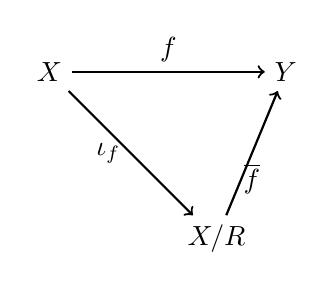
\begin{tikzpicture}[node distance=3cm, auto]
		\node (X) {\(X\)};
		\node (Y) [right of=X] {\(Y\)};
		\node (Xquot) [below right of=X] {\(X / R\)};
		
		\draw[->, thick] (X) -- node[above] {\(f\)} (Y);
		\draw[->, thick] (X) -- node[left] {\(\iota_f\)} (Xquot);
		\draw[->, thick] (Xquot) -- node[below] {\(\overline{f}\)} (Y);
		
	\end{tikzpicture}
	\label{fig:homomorphism_theorem}
\end{figure}

\textbf{Proof:}

We need to prove both directions, and start with 

\(\Leftarrow\): The existence of the function \(\iota_f\) and \(\overline{f}\) with their composition, tell us that for \(x, x' \in X\)

\[
	(\overline{f} \circ \iota_f)(x) = (\overline{f} \circ \iota_f)(x') \implies f(x) = f(x')
\]

Thus, giving us our desired equivalence relation \(R\) defined by \(x R x' \iff f(x) = f(x')\).

\(\Rightarrow\): We have an equivalence relation \(R\) defined by \(x R x' \iff f(x) = f(x')\). We now construct  
a function 

\[
	\iota_f: X \to X / R, \quad x \mapsto [x]_R
\]

We know that \(\iota_f\) is well defined by the definition of \(R\). Continuing we will construct another function

\[
	\overline{f}: X / R \to Y, \quad [x]_R \mapsto f(x)
\]

This maps each equivalence class \([x]_R\) in \(X / R\) to the corresponding element \(f(x)\) in \(Y\).
This map is also well defined, since none of our equivalence class is empty by definition, and if \([x]_R = [y]_R\), then \(f(x) = f(y)\) by the definition of \(R\).

Finally, we verify that the composition of these two functions gives us back the original function \(f\):

\[
	(\overline{f} \circ \iota_f)(x) = \overline{f}([x]_R) = f(x) = y
\]

Hence, our equivalence is proven.

\QED

\section{Counting Relations}

Given two sets \(A\) and \(B\) with \(|A| = n\) and \(|B| = m\), we can count the number of different types of relations from \(A\) to \(B\):

\begin{itemize}

	\item \emph{Total relations:} There are \(2^{n \times m}\) total relations from \(A\) to \(B\). Each of the 
		  \(n \times m\) possible ordered pairs \((a, b)\) can either be included in or excluded from the relation. This comes from the cardinality of 
		  the power set of the Cartesian product of \(A \times B\).

	\item \emph{Reflexive relations:} If \(A = B\), the number of reflexive relations is \(2^{n^2 - n}\). This is because 
		  the \(n\) diagonal pairs \((a, a)\) must be included, while the remaining \(n^2 - n\) pairs can be chosen freely.

	\item \emph{Symmetric relations:} If \(A = B\), the number of symmetric relations is \(2^{\frac{n(n+1)}{2}}\). This counts 
		  the diagonal pairs and half of the off-diagonal pairs, as each off-diagonal pair \((a, b)\) must be paired with \((b, a)\).

	\item \emph{Antisymmetric relations:} If \(A = B\), the number of antisymmetric relations is \(2^{n^2 - \frac{n(n-1)}{2}}\). 
		  This counts all pairs except for those that would violate antisymmetry.

	\item \emph{Transitive relations:} Counting transitive relations is more complex and does not have a simple closed-form formula. 
		  It often requires combinatorial methods or recursive counting techniques. 

\end{itemize}

\section{Refinement}

Let \(G\) and \(H\) be equivalence relations in \(A\). We call \(G\) a \emph{refinement} of \(H\) if 
\(G \subseteq H\); we also say that \(G\) is \emph{finer} than \(H\), and that \(H\) is \emph{coarser} than \(G\).

\subsection{Quotient Space for Refinements}

Let \(G\) and \(H\) be equivalence relations on a set \(A\) and let \(G\) be a refinement of \(H\). 
The \emph{quotient} of \(H\) by \(G\) usually denoted as \(H/G\), is a relation in \(A/G\) defined as follows: 

\[
	H/G = \{([x]_{G}, [y]_{G}) \mid (x, y) \in H\}
\]

In simpler words, it is a set of the pairs consisting of the equivalence classes of a pair \((x, y) \in H\).

\subsection{Equivalence Classes Under Refinements}

Let \(G\) and \(H\) be equivalence relations in \(A\), suppose \(G \subseteq H\). Then 
\(z \in [x]_{H} \implies [z]_G \subseteq [x]_H\).

\textbf{Proof:}

\(z \in [x]_{H}\) means that \((z, x) \in H\), then 

\begin{align*}
	y \in [z]_G	\implies (y, z) \in G \subseteq H &\implies (y, x) \in H \\ 
	&\implies y \in [x]_H
\end{align*}

Thus, \([z]_G \subseteq [x]_H\).

\QED

This can also be extended for all elements \(x \in A\), as \([x]_G \subseteq [x]_H\).

